\documentclass[a4paper,14pt]{article}
\usepackage[T1]{fontenc}
\usepackage[utf8]{inputenc}
\usepackage[english,serbianc]{babel}
\usepackage{graphicx}
\usepackage{subfig}
\usepackage{wrapfig}
\usepackage{fancyhdr}

\renewcommand{\figurename}{Слика}
\graphicspath{ {./img/} }

\title{Оперативни систем Linux}
\author{Алекса Сиришки}
\date{May 2022}

\begin{document}

\pagestyle{empty}
\begin{center}
\textbf{Гимназија „Јован Јовановић Змај“}
\\
Нови Сад
\end{center}
\vfill
\begin{center}
	\begin{large}
		\textbf{Матурски рад из Оперативних Система}
		\bigskip 
	\end{large}
	\\
	\begin{huge}
        \textbf{Оперативни систем Linux}
	\end{huge}
\end{center}
\vfill
\begin{normalsize}
Професор ментор:
\hfill
Ученик:
\\
Саша Тошић
\hfill
Алекса Сиришки IV-6
\end{normalsize}
\vfill
\begin{center}
Нови Сад, мај 2022. год.
\end{center}
\newpage

\pagestyle{plain}
\section*{ПРЕДГОВОР}
\addcontentsline{toc}{section}{ПРЕДГОВОР}
За ову тему сам се определио из више разлога. Првенствено због љубави према информационим технологијама, коју сам стекао захваљујући мојим родитељима. Други разлог је то што сматрам да је ово веома фасцинантна тема, јер обухвата комплексност које се може постићи када на једном пројекту ради читав свет. На крају, оно што ме је привукло да изаберем баш ову тему, јесте чињеница да је будућност информационих технологија слободан и бесплатан код.
\\\\
У овом раду анализираћу основне компоненте једног изузетног оперативног система, његову историју од настанка саме идеје, кроз вишедеценијски развој као и филозофски поглед на исти.
\newpage

\renewcommand{\contentsname}{САДРЖАЈ}
\addcontentsline{toc}{section}{САДРЖАЈ}
\tableofcontents
\newpage

\pagestyle{fancy}
\fancyhf{}
\lhead{Оперативни систем Linux}
\rhead{Алекса Сиришки, IV-6}
\cfoot{\thepage}

\section*{Увод}
\addcontentsline{toc}{section}{Увод}
Масачусетски технолошки институт (MIT) у сарадњи са другим компанијама направили су експериментални оперативни систем назван \textit{Multiplexed Information and Computing Service} (или скраћено Multics) 1960. године. Unics (данас UNIX) су касније створили и објавили Кен Томпсон и Денис Ричи (Слика а) из AT\&T 1970. године као сопствену верзију Multics-а. Касније је преведен у Ц програмски језик и тиме постао веома флексибилан и лако изменљив. Разни факултети и универзитети су правили своје верзије Unix-a, нпр. BSD који је попут Linux-a и данас у употреби.\cite{revos}
\\\\
Ричард Метју Столмен (Слика б), оснивач GNU пројекта\cite{gnu}, је уз свој тим започео израду комплетног оперативног система чија је главна намена била да буде отворена и слободна алтернатива за Unix. Једина ствар која је недостајала јесте кернел, сто је језгро оперативног система које служи да повеже све друге компоненте у целину.
\\\\
Линус Торвалдс (Слика в) који је био испровоциран недостатком кернела за потпуно слободан и отворен оперативни систем одлучује да напише свој сопствени. Већ је био упућен у Minix и GNU софтвер те је током студија у Финској започео пројекат назван \textit{Linux} (Слика г). У почетку је једини радио на њему, али до данас се прикључило преко 15000 програмера у развијању кернела који се састоји из више од 17 милиона линија кода\cite{linuxfoundation}.
\\\\
\begin{figure}[h]
	\centering
    \subfloat[Кен Томпсон и Денис Ричи, творци Unix-а]{{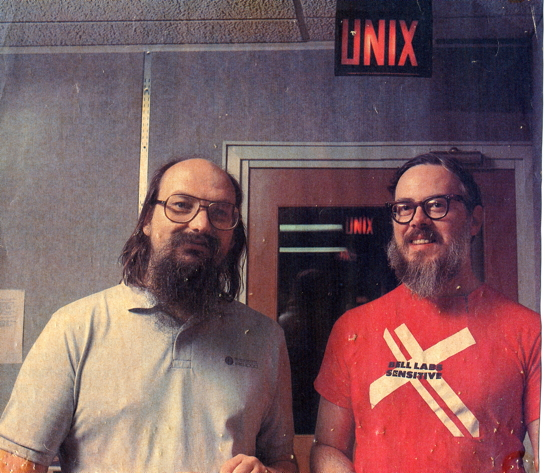
\includegraphics[height=3cm,width=4cm]{ken-thompson-dennis-ritchie} }}
    \hspace{1cm}
    \subfloat[Ричард Метју Столмен, творац GNU-а]{{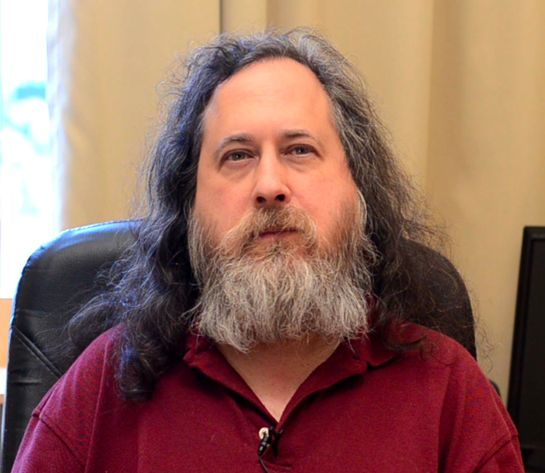
\includegraphics[height=3cm,width=4cm]{richard-stallman} }}
    \hspace{1cm}
    \subfloat[Линус Торвалдс, творац Linux-а]{{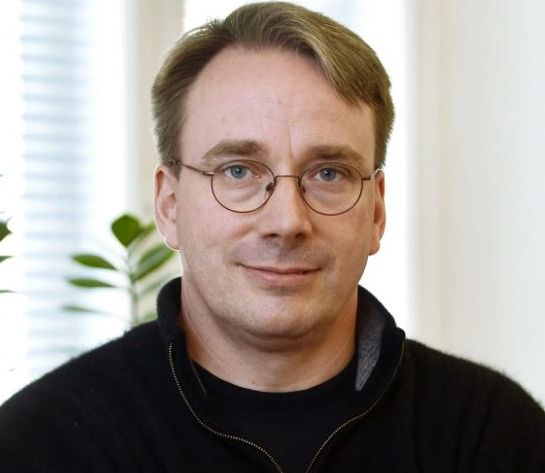
\includegraphics[height=3cm,width=4cm]{linus-torvalds} }}
    \hspace{1cm}
    \subfloat[Linux лого]{{
\includegraphics[height=3cm,width=4cm]{linux} }}
\end{figure}
\newpage

\section{ДИСТРИБУЦИЈЕ}
GNU/Linux оперативни систем се може самостално направити компајлирањем свих потребних програма (нпр. Linux From Scratch), али се најчешће користе већ готове дистрибуције. Све дистрибуције деле једну ствар, Linux кернел, али по свему осталом се могу потпуно разликовати, додуше већина дистрибуција има неке заједничке основне компоненте.
\\\\
Постоје дистрибуције прављене за сервере:
\begin{itemize}
\item Debian (Слика а)
\item Ubuntu server
\item CentOS
\item Turnkey
\end{itemize}
Као и дистрибуције прављене за десктоп кориснике:
\begin{itemize}
\item Ubuntu (Слика б)
\item Linux Mint
\item PopOS
\item Fedora Workstation (Слика в)
\end{itemize}
Такође постоје минималне дистрибуције прављене за контејнере:
\begin{itemize}
\item Alpine Linux (Слика г)
\item Fedora CoreOS
\item openSUSE MicroOS
\end{itemize}
\begin{figure}[h]
	\centering
    \subfloat[Debian]{{
\includegraphics[height=3.2cm,width=3.2cm]{debian} }}
    \hspace{1cm}
    \subfloat[Ubuntu]{{
\includegraphics[height=3.2cm,width=3.2cm]{ubuntu} }}
    \hspace{1cm}
    \subfloat[Fedora]{{
\includegraphics[height=3.2cm,width=3.2cm]{fedora} }}
    \hspace{1cm}
    \subfloat[Alpine]{{
\includegraphics[height=3.2cm,width=3.2cm]{alpine} }}
\end{figure}
\newpage

\section{КОМПОНЕНТЕ}
\subsection{Кернел}
Кернел\cite{kernel} је најважнији део сваког оперативног система. Служи да покрене сваку компоненту која је потребна за коришћење оперативног система као и да дозволи комуникацију софтвера са хардвером, или једног софтвера са другим. Кернел је неопходан да би оперативни систем функционисао и као такав је кључно да је минималан и ефикасан.

\subsubsection{Категорије кернела}
Постоје различите врсте кернела\cite{kernelcats}, неки су комплекснији али модуларнији а неки су једноставнији и бржи.
\begin{itemize}
\item Монолитски - сви сервиси оперативног система се налазе и извршавају у простору самог кернела. Тиме се одржава зависност између системских компоненти која подразумева већу комплексност кода што га чини веома захтевним за одржавање.
\begin{itemize}
\item Unix
\item Linux
\item Open VMS
\item XTS-400
\end{itemize}
\item Микрокернел - минималистички, има виртуелну меморију и распоређивање нити (енг. \textit{thread scheduling}). Самим тим што је мањи је и стабилнији, али зато има много више системских позива јер ставља све друге процесе у кориснички простор.
\begin{itemize}
\item GNU Hurd
\item Mach (MacOS)
\item L4
\item AmigaOS
\item Minix
\item K42
\end{itemize}
\item Хибридни - мешавина монолитског и микро кернела. Има брзину и дизајн монолитског али модуларност и стабилност микрокернела.
\begin{itemize}
\item Windows NT
\item Netware
\item BeOS
\end{itemize}
\item Егзокернел - прати \textit{end-to-end} принцип, има најмању апстракцију хардвера и директно додељује физичке ресурсе апликацијама.
\item Нанокернел - само апстракција хардвера, без системских сервиса. Веома сличан микрокернелу.
\end{itemize}
\newpage

\subsubsection{Делови Linux кернела}
Неки од основних делова Linux кернела\cite{devibm}:
\begin{itemize}
\item Менаџер процеса - као што му име имплицира, служи да рукује процесима тј. програмима. Сваки процес је заправо свој виртуални процесор, назван нит. Програми могу алоцирати више нити, такозваних \textit{радника}. Термин \textit{процес} и \textit{нит} су истог значења, мада је \textit{процес} популарнији у Десктоп апликацијама.
\item Менаџер меморије - меморија у Linux-у је програмима представљена као гомила страница које су потом мултиплициране и додељиване по захтеву тог програма. Стандард су странице од 4KB. Такође, странице је могуће пребацити са системске меморије на хард диск, такав поступак се назива \textit{swapping}.
\item Драјвери - код који чини највећи део Linux кернела, омогућава коришћење одређеног хардвера.
\item Виртуелни систем датотека (VFS) - апстрактује основне команде за манипулацију података чиме омогућава коришћење разноврсних система датотека.
\end{itemize}
\newpage

\subsection{Bootloader}
Bootloader је програм који се покреће пре самог оперативног система. Омогућава избор између више оперативних система (dual boot), као и избор између различитих кернела истог оперативног система. Најпре се покреће кернел, затим микрокод процесора (нпр. intel-ucode, amd-ucode) и на крају иницијални меморијски диск (\textbf{init}ial \textbf{ram} \textbf{f}ile\textbf{s}ystem). Такође, у bootloader-у се дефинишу додатне и замењиве опције за кернел.
\subsubsection{Bootloader-и са подршком за Linux}
\begin{itemize}
\item \textbf{GR}and \textbf{U}nified \textbf{B}ootloader - најпопуларнији због велике подршке за свакакве системе, једини подржава енкриптовану boot партицију. Настао као део програма за GNU оперативни систем.
\item rEFInd - настоји да има што више опција као GRUB али са мањим и једноставнијим конфигурацијама.
\item systemd-boot - део systemd, веома једноставан и минималан.
\item EFISTUB - метода уметања Linux кернела као самосталног bootloader-a у новије UEFI BIOS системе.
\end{itemize}

\subsection{Daemons}
Демони\cite{daemon}, назив настао од Максвеловог демона који у позадини сортира молекуле, служе да раде баш то: у позадини постоје без корисничког интерфејса и чекају на неки догађај и да нуде услуге.

\subsection{initramfs}
Init је први програм који се покреће након кернела, аутоматски постаје родитељ сваког наредног програма и последњи се зауставља при гашењу рачунара. Као такав, служи да омогући приступ фајл системима, да регулише демоне и снабдева информације о њима.
\subsubsection{Init системи са подршком за  Linux}
\begin{itemize}
\item systemd - најпопуларнији али и најобимнији, не прати KISS (\textit{keep it simple, stupid}) јер интегрише многобројне додатне функционалности којим инит систем не би требао да се бави.
\item OpenRC - први избор за оне које не воле сyстемд, минималан и брз.
\item GNU Shepherd - настао као део програма за GNU оперативни систем.
\item BusyBox - створен за коришћење на уграђеним слабим уређајима (енг. \textit{embedded devices}).
\item runit - UNIX init систем, замена за SysVinit.
\item SysVinit - традиционални init систем.
\end{itemize}
\newpage

\subsection{Shell}
Љуска (енг. \textit{shell}) служи да кориснику пружи искључиво текстуални интерфејс, назив \textit{љуска} упућује да је то спољни део оперативног система. Корисник уноси команде и добија одговоре. Осим покретања програма, shell може да користи излаз једне команде као улаз друге, што се назива \textit{piping} (прво уведен у UNIX-у). Такође може да се користи и као програмски језик при писању shell скрипти.
\subsubsection{Shell-ови са подршком за Linux}
\begin{itemize}
\item bash - најпопуларнији и стандард за већину дистрибуција, брз и једноставан. Настао као замена за sh.
\item zsh - обимнији и спорији, најпре се користи ради аутоматског завршавања при уносу команди и сугестије истих.
\item fish - сличан zsh-у, једноставнији за конфигурацију али није POSIX (неке основне команде се разликују од већине других shell-ова)
\item sh - UNIX shell
\item dash - минималан и ефикасан, настао искључиво да покреће POSIX скрипте. Четири пута бржи од bash-а, али није прављен за директно коришћење у терминалу.
\end{itemize}

\subsection{Дисплеј сервер}
Дисплеј сервер служи да омогући приказ GUI-а корисницима користећи WIMP (прозори, иконице, менији, показивач курсора) парадигму за кориснички интерфејс. Свака апликација добија свој прозор изменљиве величине, најчешце правоугаоног облика.
\subsubsection{Дисплеј сервери са подршком за Linux}
\begin{itemize}
\item X, X11 или XOrg - први и најкоришћенији дисплеј сервер за UNIX-оидне системе. Настао пре више од 30 година и још увек у употреби због споре адопције других протокола. Захтева додатан композитор за било какве ефекте (нпр. провидност прозора) и VSync.
\item Wayland - настао у циљу да буде модерна алтернатива за X пре више од 10 година, али је тек у протеклих пар година почео експоненционално да се развија и данас је стандард на само пар дистрибуција (Fedora, Ubuntu, openSUSE, Debian). Драстично повећава безбедност тиме што додаје контролу дозвола апликацијама, за разлику од X где свака апликација може да види једна другу. Wayland нема додатне композиторе, већ је свака примена Wayland протокола сама свој композитор.
\end{itemize}
\newpage

\section{КОМАНДЕ}
Једна од великих предности Linux оперативног система јесте терминал, којим је омогућена употреба комплетног корисничког интерфејса. Тек је накнадно убачена подршка за графички кориснички интерфејс.
\subsection{Основне команде у Linux терминалу}
\begin{itemize}
\item pwd - исписује тренутни директоријум у ком се налази и у ком ће се извршавати све команде. Иницијални терминал је кућни фолдер корисника који га покреће.
\item ls - исписује све фолдере и фајлове у задатом директоријуму. У случају скривених фолдера и фајлова користи се \textbf{ls -a}.
\item cd - мења тренутну локацију тј. фолдер.
\item mv - премешта фајл.
\item cp - копира фајл.
\item mkdir i rmdir - прави и брише фолдер (само ако је празан).
\item touch i rm - прави и брише фајл.
\item cat - исписује све што се налази унутар фајла.
\item man - исписује упутсва једне команде.
\item sudo - \textbf{S}uper \textbf{U}ser \textbf{DO} - покреће команду као root корисник.
\end{itemize}
\newpage

\section{ХИЈЕРАРХИЈА СИСТЕМА ДАТОТЕКА}
На Linux оперативном систему све је представљено као фајл - језгра процесора, системски дискови, чак и тастатура и миш. Хијерархија система датотека (FSH) дефинише структуру фолдера. Све се налази унутар главног root фолдера и приступа му се косом цртом.
\subsection{Главни директоријуми Linux система датотека}
\begin{itemize}
\item bin - неопходни програми за покретање система - mount, ls, cp.
\item boot - неопходни фајлови за покретање система - кернел, инитрамфс, микрокод процесора.
\item dev - уређаји представљени као фајлови - хард дискови, процесор, графичка картица.
\item etc - конфигурациони фајлови за системске програме.
\item home - фолдери и фајлови свих корисника на систему са изутетком главног корисника на /root.
\item lib - библиотеке потребне за покретање програма из /bin.
\item media - место за прикључне медије, нпр. usb flash, CD.
\item mnt - слично /media, намењено за приступ привременим уређајима.
\item proc - информације о системским процесима и кернелу у облику фајлова.
\item tmp - привремени фајлови који се бришу при гашењу рачунара.
\item usr - примарни директоријум за извршавајуће програме на систему.
\item var - променљиви фајлови који записују промене и податке током извршавања програма.
\end{itemize}
\newpage

\section{ДОЗВОЛЕ И ВЛАСНИШТВО}
Linux оперативни систем за сваки објекат, тј. фајл или фолдер, има одређене дозволе. Могуће их је видети командом \textbf{ls -l}. Постоје три врсте дозвола: читање, писање и покретање. Такође постоје три врсте власништва: власник, група и сви остали. На та три власнишва се одређује које дозволе имају, користећи следеће бројеве (поред којих је приказ у бинарном систему ради лакшег разумевања):
\begin{itemize}
\item 0 - 000 - нема никаквих дозвола
\item 1 - 001 - дозвола за покретање
\item 2 - 010 - дозвола за писање
\item 3 - 011 - дозвола за покретање и писање
\item 4 - 100 - дозвола за читање
\item 5 - 101 - дозвола за читање и покретање
\item 6 - 110 - дозвола за читање и писање
\item 7 - 111 - има све дозволе
\end{itemize}
Дозволе (Слика а) неког фајла или фолдера се мењају командом \textbf{chmod} а власништво командом \textbf{chown vlasnik:grupa}.
\begin{figure}[h]
	\centering
    \subfloat[Дозволе]{{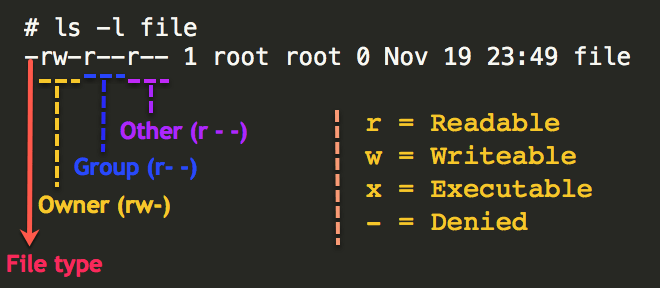
\includegraphics[height=4cm,width=10cm]{dozvole} }}
\end{figure}
\newpage

\section{ОКРУЖЕЊА РАДНЕ ПОВРШИНЕ}
Окружења радне површине су скупови програма који омогућавају коришћење графичког интерфејса. Чине их разне компоненте као што су менаџер пријава, закључавајући екран, текстуални едитор и најважније менаџер прозора. Могуће је имати само менаџер прозора и засебно скидати све друге потребне програме за коришћење графичког интерфејса али коришћење комплетног окружења драстично поједностављује тај процес.
\subsection{Окружења радне површине са подршком за Linux}
\begin{itemize}
\item GNOME\cite{gnome} (Слика а) - GNU окружење са подршком за Wayland, најпопуларнији избор за дистрибуције. Настао као део програма за GNU оперативни систем.
\item KDE Plasma\cite{kdeplasma} (Слика б) - друго најпопуларније окружење, такође са подршком за Wayland. Настао као више изменљиво окружење које је мери са GNOME који има специфични филозофски поглед на начин употребе рачунара.
\item Xfce\cite{xfce} - модуларно и незахтевно окружење.
\item LXQt\cite{lxqt} - окружење које користи најмање ресурса.
\item MATE\cite{mate} - започет као клон GNOME 2 када је GNOME прешао на верзију 3, али сада и сам користи ту верзију.
\end{itemize}
\begin{figure}[h]
	\centering
    \subfloat[GNOME]{{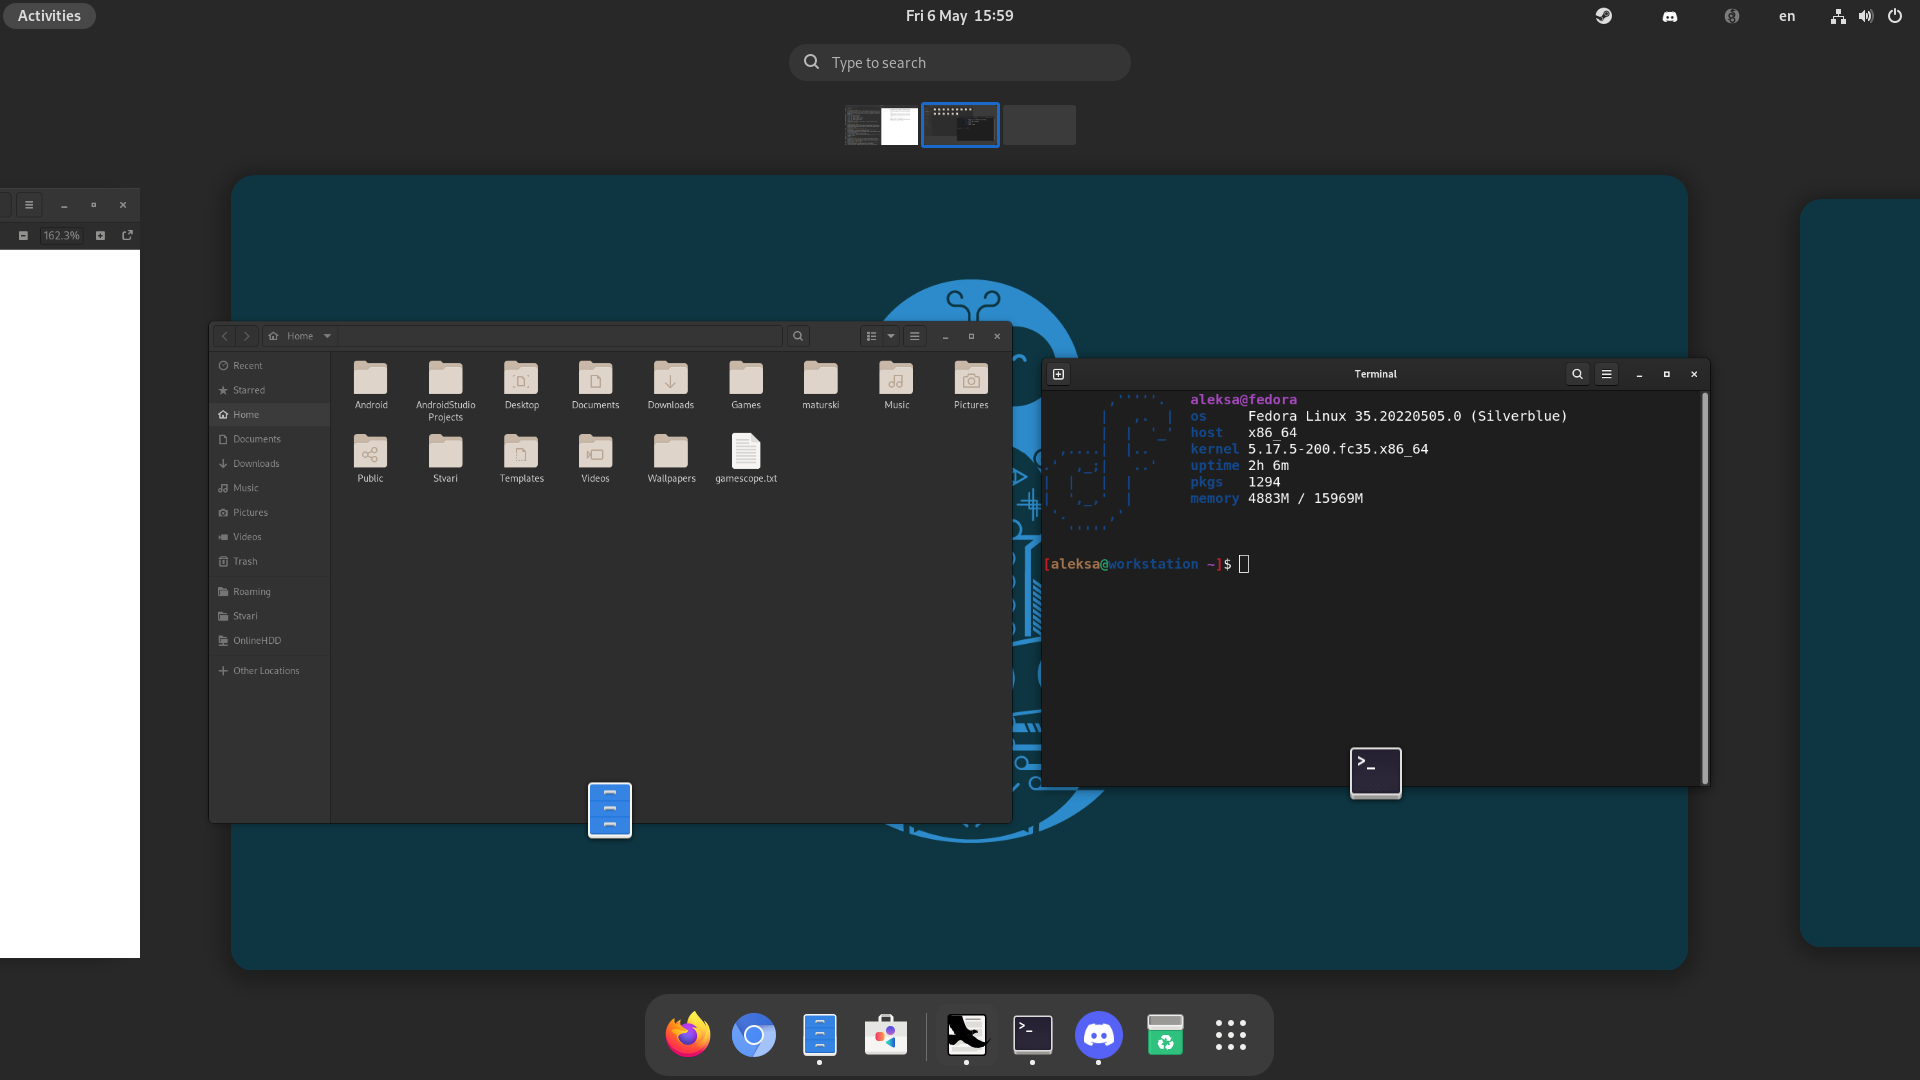
\includegraphics[height=4.4cm,width=8cm]{gnome} }}
    \hspace{0.5cm}
    \subfloat[KDE Plasma]{{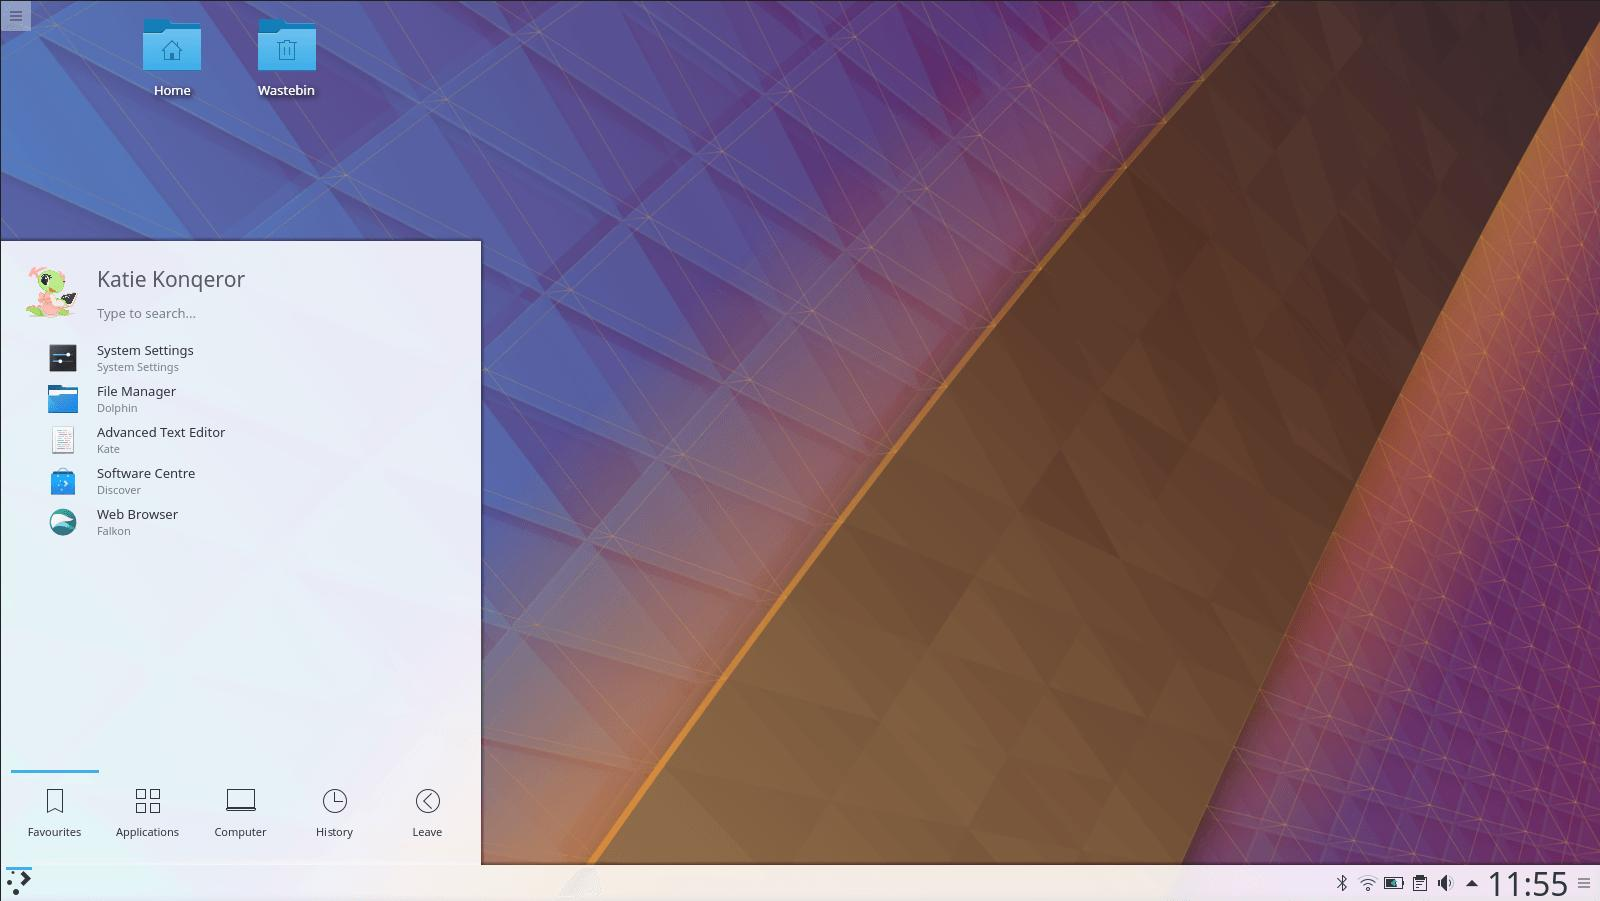
\includegraphics[height=4.4cm,width=8cm]{kdeplasma} }}
\end{figure}
\newpage

\section{КОНТЕЈНЕРИЗАЦИЈА}
Контејнеризација је једна од јачих страна Linux оперативног система. Могућност изолације програма од остатка система са минималним губитком перформанси је разлог зашто је Linux избор за највећи број сервера. За разлику од виртуелних машина, контејнери деле кернел са домаћим оперативним системом и тиме штеде на величини.
\subsection{Врсте контејнерских окружења}
\begin{itemize}
\item Linux контејнери\cite{lxc} - најпростији вид коришћења контејнера на Linux-у, помоћу cgroups из кернела омогућено је креирање више контејнера на једном домаћину.
\item Docker\cite{docker} - најпримењивији бесплатан софтвер за манипулацију контејнера.
\item Podman\cite{podman} - RedHat-ова алтернатива за Docker, настоји да буде синтаксно идентична али не захвета root дозволе за разлику од Docker-a.
\item Flatpak\cite{flatpak} - RedHat-ова једноставна дистрибуција десктоп апликација коришћењем контејнера. Девелопери могу предвидљиво да праве контејнер поред сопствене апликације и тако осигуравају да ће се она идентично понашати независно од домаћинског оперативног система. Успут пружа огромна побољшања за безбедност у виду дозвола (слично Android-у).
\item Snap\cite{snap} - Canonical-ова дистрибуција апликација, слична flatpak-у али тренутно много спорија. Серверска страна им је централизована и затвореног кода.
\item AppImage\cite{appimage} - настоји да олакша дистрибуцију апликације као flatpak и snap, али нема једно место на ком се налазе апликације, већ девелопери сами праве и дистрибуирају налик обичним покретљивим датотекама (нпр. exe, deb, rpm). Свака апликација долази уз свој скуп библиотека и програма потпуно изолованих, што беспотребно троши меморију, али је лакше за одржавање.
\end{itemize}
\newpage

\section{ПРИМЕНА}
Linux оперативни систем је први избор за највећи број сервера због своје добро познате стабилности и модуларности као и професионалној подршци од стране RedHat\cite{redhat}.
\begin{itemize}
\item 90\% јавних cloud операција се извршава на Linux-у.
\item 54.2\% суперкомпјутера користи Linux од којих 500 најјачих на свету користе искључиво Linux.
\item Сваки Android уређај користи Linux кернел, што укључује и Android паметне сатове и телевизоре.
\item Паметни телевизори који немају Android оперативни систем најчешће користе своју дистрибуцију Linux-а (нпр. Tyzen од Samsung-а).
\item 83.1\% професионалних програмера сматрају Linux као најбољу платформу за развијање програма.
\item 90\% свих Холивудских специјалних ефекета су створени на Linux-у.
\end{itemize}
Поред свих ових употреба Linux је такође коришћен и у разним научним (нпр. \textit{Machine Learning}) и образовним институцијама (нпр. ChromeOS\cite{chromeos}).
\\\\
Једино место где Linux још увек није засијао је на Десктоп рачунарима где се убраја у само 3.37\%. Разлог за то је огромна затвореност студија за производњу игрица и тврдоглавост компанија као што су Microsoft и Adobe да своје продукте учине покретљивим на Linux-у.
\newpage

\section*{Закључак}
\addcontentsline{toc}{section}{Закључак}
Упркос томе што се базира на бесплатном моделу постојањем компанија као што су RedHat и мноштвом спонзора (Microsoft, Google, Meta) Linux наставља да се експоненцијално развија. Програмери иза Linux-а имају приходе налик програмерима идентичних производа затвореног кода, што доказује да је етика слободног кода успешна и да не постоји разлог за затвореним кодом осим прикупљања персоналних података без јавног признања о том поступку. Важно је напоменути да ако је нешто \textit{отворен} код не значи и да је \textit{слободан} код. Отворен код дозвољава свакоме да види тачно шта се извршава у програму али му не даје на право да ради са тим кодом шта год пожели, док слободан код омогућује свакоме да поново користи тај код за нешто потпуно друго ако ће такође дозволити поновну употребу тог новонасталог кода. Тиме се драстично смањује потреба за писањем истог кода изнова. Да би се спречила крађа и злоупотреба Столмен је осмислио лиценце за отворен и слободан код (нпр. GNU General Public License\cite{gpl}).
\\\\
У данашње време просечни корисник који није и не жели да буде упућен у комплексне токове рада рачунара може врло једноставно да користи Linux употребом готових дистрибуција и успут покрене већину Windows програма захваљујући слоју компатибилности попут WINE-а\cite{wine} и VALVE-овог\cite{valve} PROTON-а\cite{proton}. Брзином развоја и распрострањеношћу подршке хардвера и софтвера врло је вероватно да ће у ближој будућности Linux заменити и тренутно главне Десктоп оперативне системе.
\newpage

\renewcommand\refname{Литература}
\addcontentsline{toc}{section}{Литература}
\bibliographystyle{unsrt}
\bibliography{literatura}
\newpage

\section*{БИОГРАФИЈА МАТУРАНТА}
\addcontentsline{toc}{section}{БИОГРАФИЈА МАТУРАНТА}
\begin{wrapfigure}{r}{0.35\textwidth}
\centering
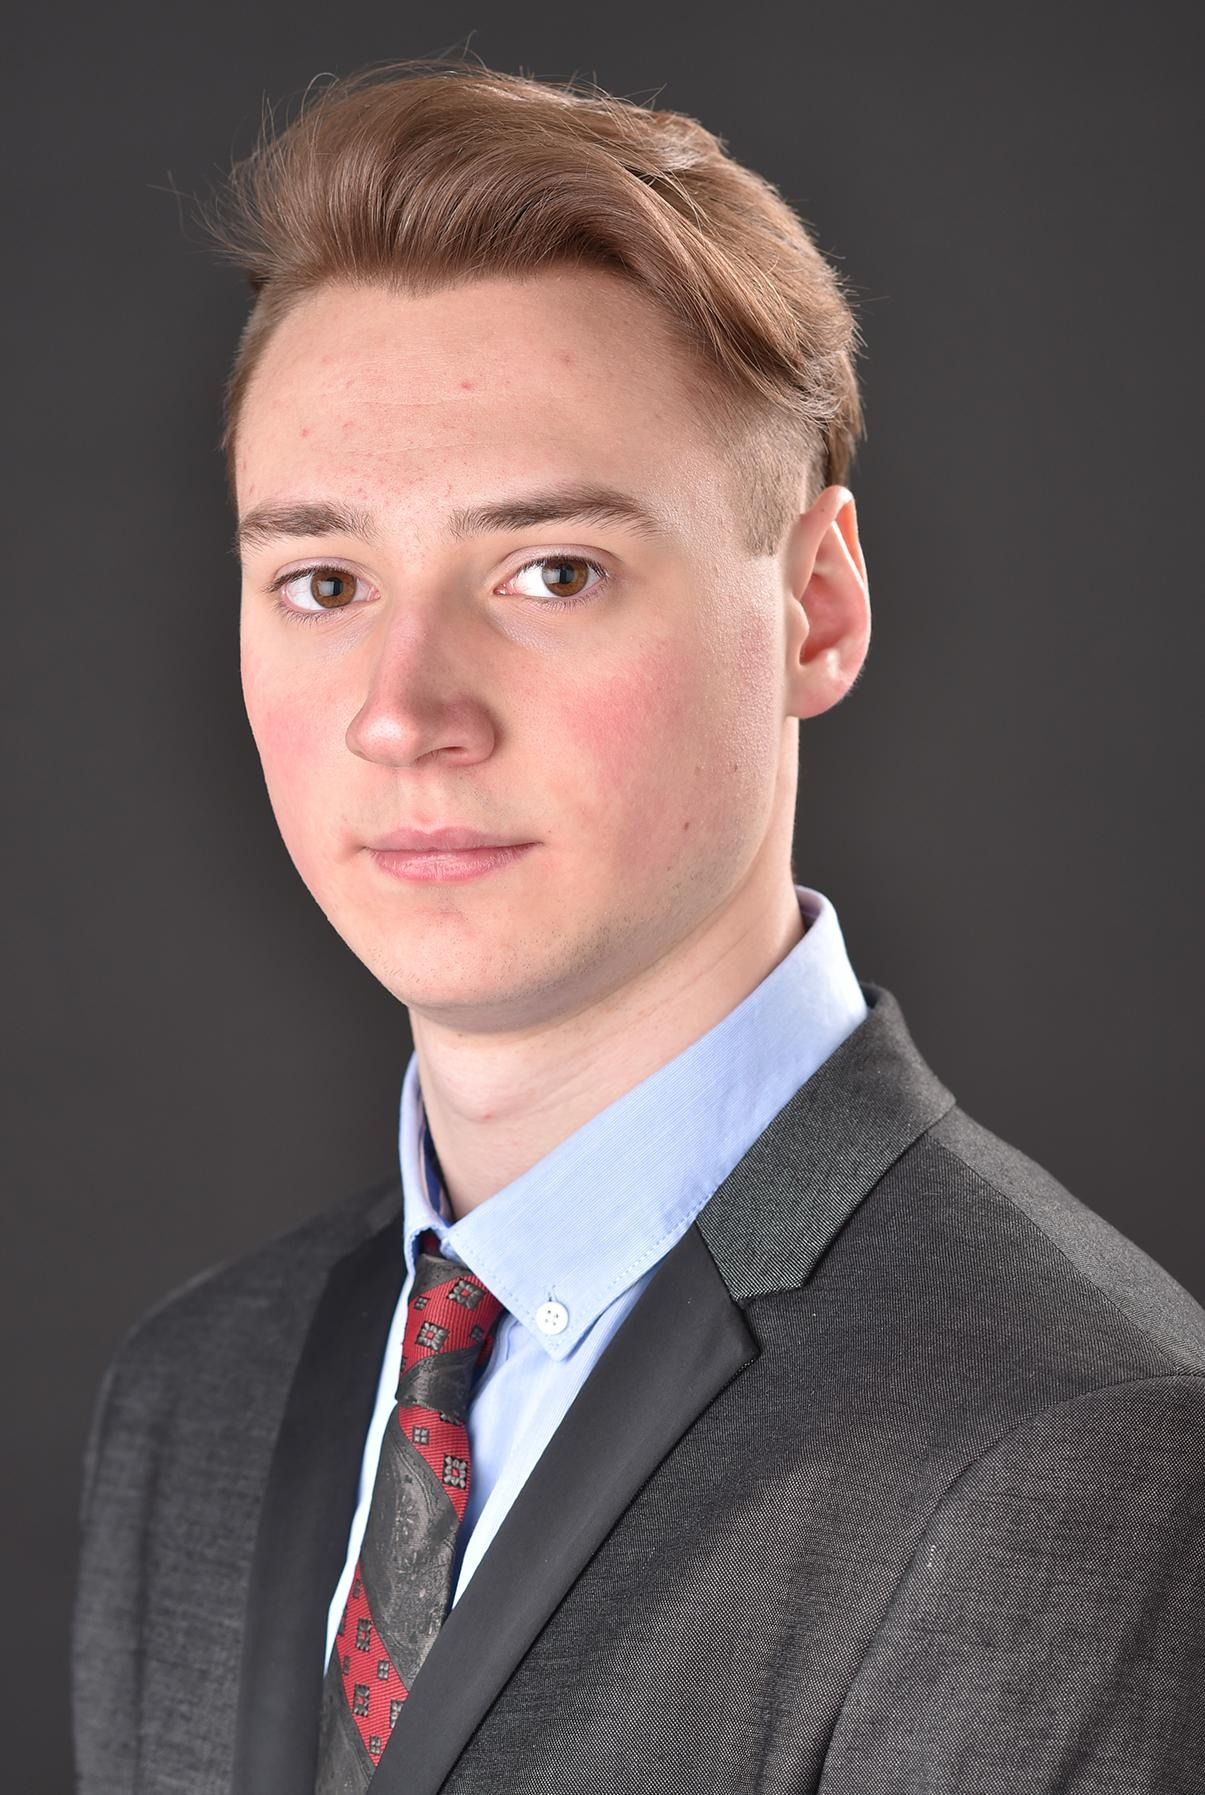
\includegraphics[width=.90\linewidth]{Maturska}
\end{wrapfigure}
Алекса Сиришки рођен је 10. јула 2003. године у Новом Саду. Похађао је Основну школу „Светозар Марковић Тоза“ до шестог разреда. Тамо стиче интересовање за математику, информатику, физику и језике. Септембра 2016. уписује Основну школу при Гимназији „Јован Јовановић Змај“, како би интензивније радио у областима математике, физике и информатике. Истовремено похађа програмерски курс „Центар за младе таленте“. Школовање наставља у истој гимназији и опредељује се за смер „Ученици са посебним способностима за рачунарство и информатику“. Наредне четири године, упоредо са школом, похађа и курсеве енглеског и немачког језика. Планира да више образовање стекне на Природно математичком факултету, смер Информационе технологије.
\newpage

\newcommand{\linija}{\noindent\underline{\makebox[3cm][t]{}}}
\newcommand{\linijamala}{\noindent\underline{\makebox[1cm][t]{}}}
\newcommand{\komentar}{\framebox(10cm,5cm)[t]{}}
\newcommand{\poravnanje}{\makebox[5cm][t]{}}
\newcommand{\prazan}{\makebox[0cm][t]{}}

\prazan \\
Датум предаје матурског рада: \linija
\\\\\\\\\\
Комисија:
\begin{quote}
Председник \hfill \linija \poravnanje
\\\\
Испитивач \hfill \linija \poravnanje
\\\\
Члан \hfill \linija \poravnanje
\end{quote}
\prazan \\\\\\
Коментар: 
\\ \prazan \hfill \komentar
\\\\\\\\\\\\\\
Датум одбране: \linija \hfill Оцена \linija (\linijamala)

\end{document}